%%%% CAPÍTULO 2 - REVISÃO DA LITERATURA (OU REVISÃO BIBLIOGRÁFICA, ESTADO DA ARTE, ESTADO DO CONHECIMENTO)
%%
%% O autor deve registrar seu conhecimento sobre a literatura básica do assunto, discutindo e comentando a informação já publicada.
%% A revisão deve ser apresentada, preferencialmente, em ordem cronológica e por blocos de assunto, procurando mostrar a evolução do tema.
%% Título e rótulo de capítulo (rótulos não devem conter caracteres especiais, acentuados ou cedilha)
\chapter{Referencial te\'orico}\label{cap:referencialTeorico}

Esta seção será dedicada a explicar como funcionam as várias partes envolvidas na construção e funcionamento de um multímetro digital e/ou multimedidor.

% RAFAEL --------------------------------------------------------------------------------------------------------

\section{Proteção de Entrada}\label{sec:InputProtection}

Proteção de entrada é um assunto extremamente abrangente quando se trata de circuitos eletrônicos. Dependendo da função que este tenha que exercer, existem infinitas topografias que podem ser consideradas. Algumas exigências, porém, são comuns, como a necessidade de um circuito de proteção contra descargas eletrostáticas, ou \gls{ESD} (\textit{Electrostatic Discharge}). Tais descargas podem entregar picos de tensão extremamente altos, chegando até a 30 kV, o que é extremamente danoso a qualquer circuito que use semicondutores. Pulsos de pico tão alto quanto 2500 V (Volts) já são o suficiente para danificar a maioria dos circuitos eletrônicos. Notoriamente, seres humanos são capazes de entregar descargas de até 20 kV por consequência da capacitância inata à sua fisiologia. \cite{ONsemicondTVS2} %%citar o documento http://www.reallyreallyrandom.com/zener/media/Zener_Theory_and_Design.pdf, página 65

    \subsection{ESD}\label{subsec:electrostaticDischarge}
    Esse tipo de proteção é necessária para circuitos que fazem interface com o meio físico e normalmente é exercida por um circuito básico de componentes \gls{TVS} (\textit{Transient Voltage Suppressor}). Os dispositivos semicondutores mais simples (e também regularmente) utilizados para exercer esta função são diodos Zener. \cite{IPblog}
    
    Ao serem submetidos a uma tensão maior que à especificada como limite de operação do circuito a ser protegido, diodos Zener apresentam uma resistência baixa, fechando a passagem de corrente entre o circuito e o ground do equipamento. Este circuito pode apresentar uma configuração unidirecional ou bidirecional, dependendo da necessidade do circuito a ser protegido. \cite{TIESD}
    
    As figuras \ref{fig:tvsUnidirecional} e \ref{fig:tvsBidirecional} demonstram a utilização básica de tal circuito e o conceito por trás da tensão de ruptura de tal semicondutor.

    \begin{figure}[htb]%% Ambiente figure
        %\captionsetup{width=0.55\textwidth}%% Largura da legenda
        \caption{Exemplo de uso TVS Unidirecional}%% Legenda
        \label{fig:tvsUnidirecional}%% Rótulo
        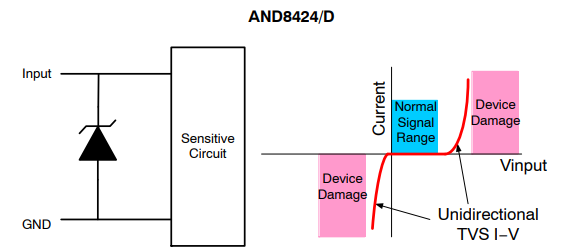
\includegraphics[scale=0.8]{tvs-unidirectional}%% Dimensões e localização
        \fonte{\cite{ONsemicondTVS}}%% Fonte
    \end{figure}

    \begin{figure}[htb]%% Ambiente figure
        %\captionsetup{width=0.55\textwidth}%% Largura da legenda
        \caption{Exemplo de uso TVS Bidirecional}%% Legenda
        \label{fig:tvsBidirecional}%% Rótulo
        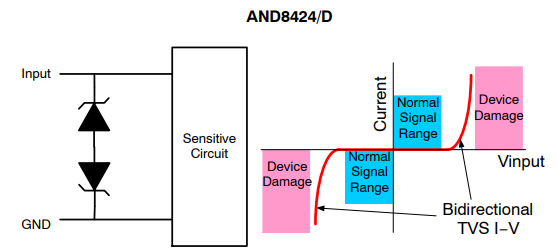
\includegraphics[scale=0.8]{tvs-bidirectional}%% Dimensões e localização
        \fonte{\cite{ONsemicondTVS}}%% Fonte
    \end{figure}

    \subsection{Proteção Específica para Equipamentos de Medição de Sinais Elétricos}\label{subsec:especProtec}

    Primeiramente, se faz necessário explicar sobre a classificação de proteção em relação a equipamentos elétricos. A classificação mais robustamente utilizada é a CAT, que vai de CAT I a CAT IV. Os numerais indicam o potencial de energia que o sistema pode entregar caso ocorra um curto-circuito ou um transiente de tensão, \textit{i.e.} um instrumento CAT III tem que estar protegido contra transientes muito maiores que um dispositivo CAT II.  

    Dispositivos CAT IV devem estar protegidos a nível de distribuição de energia, pois estes serão utilizados em conexão entrada de energia de uma facilidade. Dispositivos CAT III devem estar protegidos a nível de distribuição interna (quadros de distribuição), podendo esta ser trifásica ou monofásica. Dispositivos CAT II devem estar protegidos a nível de equipamento terminal ou de uso comum, sendo estes eletrodomésticos e afins. Dispositivos CAT I devem estar protegidos a nível de circuitos eletrônicos e transformadores de baixa potência. \cite{CATratingu} %%ref: https://www.ecmweb.com/test-measurement/article/21247639/understanding-the-cat-rating-system

    \begin{figure}[htb]%% Ambiente figure
        %\captionsetup{width=0.55\textwidth}%% Largura da legenda
        \caption{Ilustração da Classificação CAT}%% Legenda
        \label{fig:CATrating}%% Rótulo
        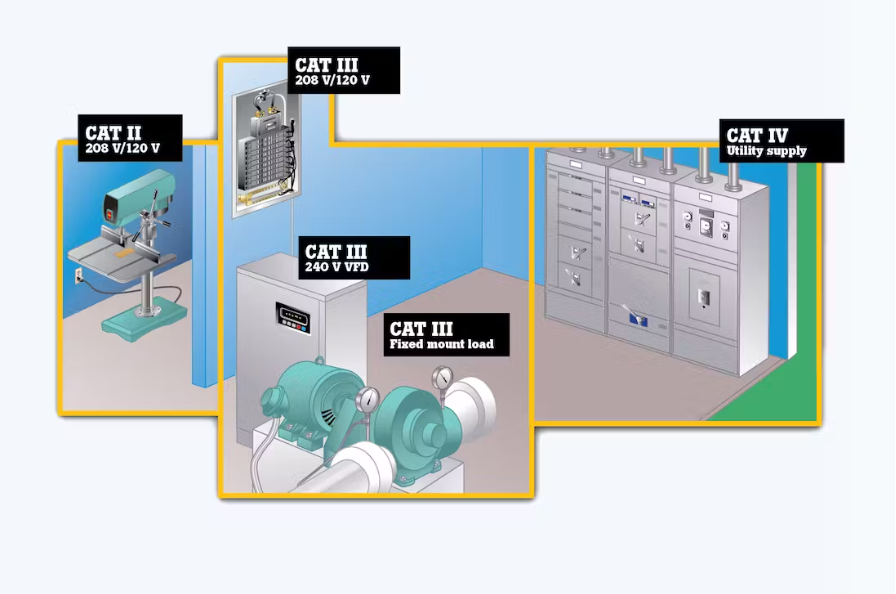
\includegraphics[scale=0.4]{CATrating}%% Dimensões e localização
        \fonte{\cite{CATratingu}}%% Fonte
    \end{figure}


    
        \subsubsection{Proteção de Entrada para Circuitos de Corrente}\label{subsec:protecaoCorrente}

        O circuito de proteção para a entrada de correntes se divide em duas partes, sendo uma delas para o range de A (Amperes) e os ranges de mA e µA.

	    Para a entrada de Amperes, é utilizado um fusível \gls{HRC} (\textit{High Rupturing Capacity}), geralmente de 11 A e 1000 V (para se adequar à classificação CAT III, no caso do multímetro que foi estudado), para se prevenir arcos voltaicos após a queima do fusível, negando a possibilidade de uma continuação da condução de curto-circuito ou sobrecorrente. Logo após, é conectado um shunt de quatro terminais, 0R005 $\Omega$, entre o ground e a entrada, no qual será feita a medida.

	    Para a entrada de mA e µA, também é utilizado um fusível \gls{HRC}, mas de 500 mA e 1000 V. Em sequência, é colocado um retificador em ponte de diodos entre o canal e o ground, para dar clamp em possíveis sobretensões (normalmente ocasionada pela utilização errônea do equipamento, colocando-se a entrada de corrente para medir tensão) até que o fusível possa atuar. Internamente, há um switch entre mA e µA. \cite{fluke27manual}

        Para o switch de mA, é conectado em série um resistor shunt de 4R995 $\Omega$ com o shunt do range de A (0R005 $\Omega$), para ser feita a medição em uma resistência total de 5 $\Omega$.

        Para o switch de µA, é conectado um resistor shunt de 500 $\Omega$, no qual será feita a medição. \cite{IPblog}%%ref: https://lygte-info.dk/info/DMMDesignProtection%20UK.html

        \subsubsection{Proteção de Entrada para Circuitos de Tensão}\label{subsec:protecaoTensao}

        O circuito de proteção para a entrada de tensão é simples, sendo este composto de um resistor \gls{WW} (WireWound) em série com um termistor \gls{PTC} (\textit{Positive Temperature Coefficient}) em série com um resistor de 10 M$\Omega$, no qual será feita a medida. \cite{fluke27manual}

        Conectado em paralelo ao resistor de 10 M$\Omega$ com o ground input, há uma série de varistores \gls{MOV} (\textit{Metal Oxide Varistor}) de rápida atuação como proteção para transientes de sobretensão, até que o termistor consiga esquentar. Pode ser utilizado somente um varistor, mas uma série destes aumenta a distância de fuga de corrente, reduzindo a chance de arcos voltaicos e também dissipando energia entre vários componentes, melhorando a proteção. \cite{flukeblog}

        Uma parte importante do design geral da \gls{PCB} (\textit{Printed Circuit Board}) são slots de isolamento de alta tensão, que se resumem a espaços abertos entre partes da placa, que vão receber altas tensões em funcionamento indesejado, para minimizar as chances de arcos voltaicos entre partes do circuito, como explícito na \autoref{fig:exemploPCB}. %%ref: https://lygte-info.dk/info/DMMDesignProtection%20UK.html

        \begin{figure}[htb]%% Ambiente figure
            %\captionsetup{width=0.55\textwidth}%% Largura da legenda
            \caption{Fluke 28-II PCB}%% Legenda
            \label{fig:exemploPCB}%% Rótulo
            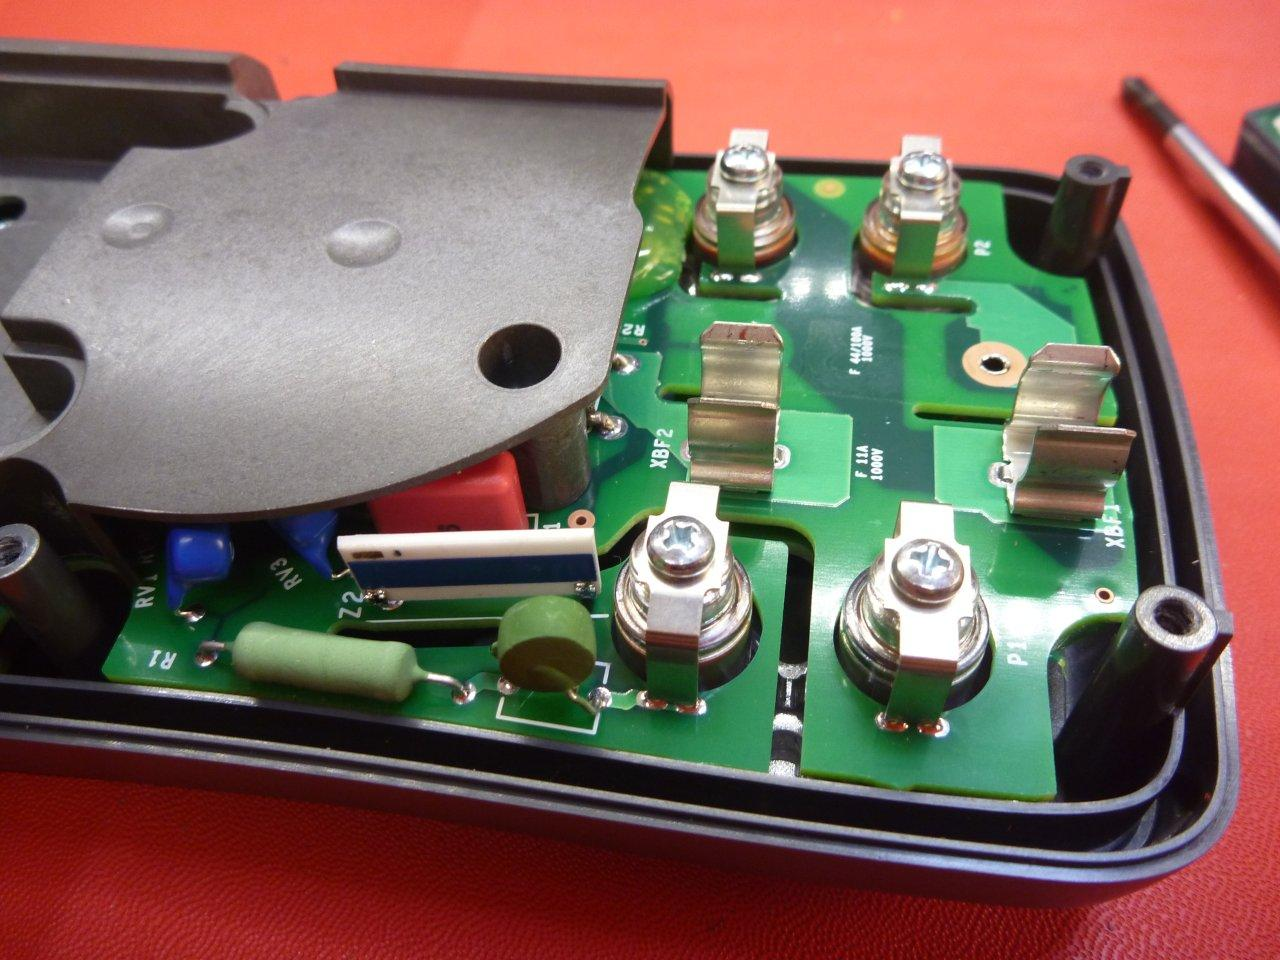
\includegraphics[scale=0.6]{divetPCB}%% Dimensões e localização
            \fonte{\cite{flukeforum}}%% Fonte
        \end{figure}    

\section{Conversor Analógico Digital}\label{sec:ADC}

O \gls{ADC} (\textit{Analog-to-Digital Converter}) é uma parte integral do funcionamento dos equipamentos de medição elétrica, pois este fará o interfaceamento, ou seja, a leitura do sinal analógico a ser interpretado e o converterá para um sinal digital que pode assim ser processado, como mostrado na \autoref{fig:ADCDB}.

\begin{figure}[htb]%% Ambiente figure
    %\captionsetup{width=0.55\textwidth}%% Largura da legenda
    \caption{Diagrama de blocos de um ADC}%% Legenda
    \label{fig:ADCDB}%% Rótulo
    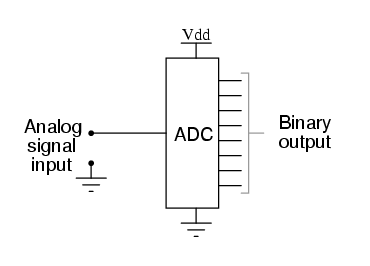
\includegraphics[scale=0.8]{ADCDB}%% Dimensões e localização
    \fonte{\cite{ADCbook}}%% Fonte: Lessons in Electric Circuits: Volume IV - Digital, by Tony R. Kuphaldt
\end{figure}  

Existem vários tipos de \gls{ADC}s, sendo alguns deles:

\begin{itemize}
    \item \textit{Flash} \gls{ADC};
    \item \textit{Digital Ramp} \gls{ADC};
    \item \textit{Successive Approximation} \gls{ADC};
    \item \textit{Tracking} \gls{ADC};
    \item \textit{Slope (integrating)} \gls{ADC};
    \item \textit{Delta-Sigma ($\Delta$ $\Sigma$)} \gls{ADC};
    \item entre outros\dots
\end{itemize}

Para fins de objetividade, será somente apresentado o \gls{SAR} (\textit{Successive Approximation Register}), pois este é o mais comumente utilizado em multímetros e o \gls{ADC} mais básico, chamado de \textit{Flash}. Porém, dependendo da aplicação e necessidade de resolução ou precisão, são utilizados outros tipos de \gls{ADC} também.

    \subsection{Flash ADC}\label{flashADC}

    Este \gls{ADC} delimita o principio de funcionamento desse tipo de dispositivo. Formado de uma série de comparadores, como mostrado na \autoref{fig:flashADC}, este compara o sinal de entrada com uma tensão de referência única para cada comparador. A saída destes comparadores são conectadas à um \textit{encoder} de prioridade que produz uma saída binária. 
    Esta topologia não só é a mais simples em termos de operação, mas também é o mais eficiente, em termos de velocidade, sendo limitado só pelos comparadores e \textit{delays} de propagação dos gates. Infelizmente, o \textit{flash} \gls{ADC} necessita de um número excessivo de componentes, sendo necessários 255 comparadores para uma saída de 8-bits, que seria a necessidade de \textit{output} de qualquer \gls{ADC} moderno. 

    \begin{figure}[htb]%% Ambiente figure
        %\captionsetup{width=0.55\textwidth}%% Largura da legenda
        \caption{Diagrama de blocos de um ADC Flash}%% Legenda
        \label{fig:flashADC}%% Rótulo
        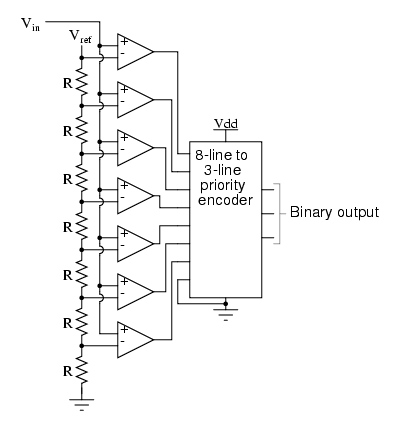
\includegraphics[scale=0.8]{flashADC}%% Dimensões e localização
        \fonte{\cite{ADCbook}}%% Fonte: Lessons in Electric Circuits: Volume IV - Digital, by Tony R. Kuphaldt
    \end{figure}  

    \subsection{SAR ADC}\label{SARADC}
    O \gls{SAR} funciona de maneira que se é conectado um contador \gls{SAR}, que faz uma contagem testando todos os valores de bits, começando com o mais significativo e terminando com o menos significativo a um \gls{DAC} que então sua saída é comparada com o sinal analógico a ser obtido. 
    
    Durante o processo de contagem, um registro monitora a saída deste comparador para ver se a contagem binária é maior ou menor que a entrada do sinal analógico, ajustando os valores de bit de acordo. A maneira que este registro conta é idêntica ao método de conversão decimal para binário, portanto diferentes valores de bits são testados do bit mais significante ao menos significante para conseguir um número binário que se iguala ao número decimal original. 

    O circuito e resultado de leitura do \gls{ADC} em questão, em termos simples, pode ser representado pelas figuras \ref{fig:SARADC} e \ref{fig:SARADCplot}.

    \begin{figure}[htb]%% Ambiente figure
        %\captionsetup{width=0.55\textwidth}%% Largura da legenda
        \caption{Diagrama de blocos de um ADC SAR}%% Legenda
        \label{fig:SARADC}%% Rótulo
        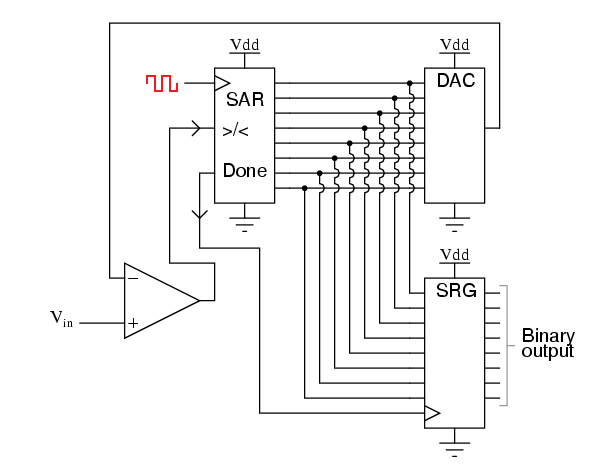
\includegraphics[scale=0.8]{SARADC}%% Dimensões e localização
        \fonte{\cite{ADCbook}}%% Fonte: Lessons in Electric Circuits: Volume IV - Digital, by Tony R. Kuphaldt
    \end{figure}  

    \begin{figure}[htb]%% Ambiente figure
        %\captionsetup{width=0.55\textwidth}%% Largura da legenda
        \caption{Plot sobre o tempo da saída de um ADC SAR}%% Legenda
        \label{fig:SARADCplot}%% Rótulo
        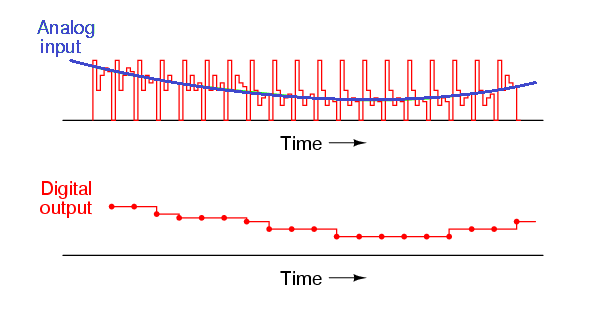
\includegraphics[scale=0.8]{SARADCplot}%% Dimensões e localização
        \fonte{\cite{ADCbook}}%% Fonte: Lessons in Electric Circuits: Volume IV - Digital, by Tony R. Kuphaldt
    \end{figure} 


\section{Calibração}\label{sec:Calibration}

Todo equipamento de medição precisa ser calibrado para exercer a sua função com precisão. Normalmente, este serviço é feito pelo provedor do produto e, dependendo do tipo de uso de tal produto e sua precisão, feito em intervalos regulares para garantir sua eficácia. Muitas vezes, realizar a calibração de um equipamento como um multímetro pode ser mais caro que comprar um novo.

Para se calibrar um multímetro, é utilizado um outro dispositivo com no mínimo 4x a precisão do multímetro a ser calibrado. Portanto, normalmente se é utilizado um equipamento específico para exercer tal função. Esse equipamento geralmente é chamado de \textit{calibrator} ou \textit{standard}. \cite{flukecalib} %ref: https://eu.flukecal.com/products/electrical-calibration-0

Tais equipamentos também necessitam ser calibrados, então o fornecedor deve garantir que estes estejam de acordo com os órgãos regionais, nacionais e internacionais em questão de procedência da calibração. Uma documentação e traçabilidade extensivas são requerimentos indispensáveis.

    \subsection{Calibrators ou Standards}\label{subsec:Calibrators}

    O \textit{calibrator} tem a capacidade de fornecer sinais elétricos precisos e de função variável, que podem ser produzidos de µV a kV, normalmente. Estes sinais, em ranges específicos, serão lidos pela \gls{UUT} (\textit{Unit Under Test}) e então serão anotados os resultados da medição, fazendo-se um levantamento de dados do multímetro. Após tal levantamento, realiza-se os passos necessários para calibrar tal dispositivo, dependendo das suas necessidades e também do fabricante do mesmo. Este equipamento também consegue fazer medições de precisão, caso seja necessário. 

    O \textit{standard} cumpre a mesma função do calibrator, mas geralmente é limitado a poucos ranges de geração de sinal e somente uma função, o que possibilita uma performance e precisão muito maior que a do \textit{calibrator}. 

Entretanto, existe uma proposta de calibração do equipamento on-board, feita pela \gls{TI} (\textit{Texas Instruments}), utilizando-se um \gls{DAC} para corrigir erros de leitura, seja por mudanças de temperatura, mudança na tensão de referência do \gls{ADC} ou qualquer outro fator que possa afetar a leitura do sinal. Também nesse circuito é incluído um sensor de temperatura para avisar o usuário sobre mudanças consideráveis de temperatura.

O funcionamento do \gls{DAC}, porém, está diretamente relacionado à sua tensão de referência. Geralmente, se é utilizada uma referência externa para medidas de precisão, pois esta estará isolada da aquisição de sinal do multímetro e logo não será afetada caso haja uma mudança de temperatura. \cite{analogdac} A solução proposta pela \gls{TI} é de se utilizar um \gls{DAC} de precisão (16-Bits) com \textit{on-board low-drift voltage reference} junto com um \textit{buffer} por meio de um \gls{amp-op} de alta velocidade. Tais componentes são de uso extremamente específico e por isso são caros, colocando-os assim fora do escopo do estudo desta presente tese. \cite{DACTI} %ref: https://www.analog.com/en/analog-dialogue/articles/buffering-the-output-of-high-speed-dacs.html e https://www.ti.com/lit/ug/tiduct8/tiduct8.pdf?ts=1685988821918&ref_url=https%253A%252F%252Fwww.ti.com%252Fsolution%252Fdigital-multimeter-dmm%253Fvariantid%253D20220%2526subsystemid%253D33430

\section{Referência de Tensão}\label{sec:VoltageReference}

A referência de tensão do ADC, utilizada para a leitura do sinal analógico, pode estar incluída no chip, que é uma solução mais barata e de menor precisão para equipamentos que não exigem tal afinidade, ou ser externa ao chip, que provém uma melhor precisão e, consequentemente, uma melhor leitura. Tal referência externa, hodiernamente, é feita por um \gls{CI} (Circuito Integrado) especializado, como por exemplo o ICL8069 \cite{icl8069}, visto sendo utilizado no estado da arte. %datasheet: https://pdfserv.maximintegrated.com/en/ds/ICL8069.pdf


\section{Condicionamento de Sinal e Pathing}\label{sec:signalConditioningandPathing}

O condicionamento de sinal se resume ao controle da entrada apropriada a ser avaliada pelo ADC, que geralmente é feita por um \gls{MUX} (Multiplexador), por \textit{switches} mecânicos, como exemplificado na \autoref{fig:Fluke28-II-switches}, ou em alguns casos, por uma combinação dos dois.  \cite{dmmblog}

\begin{figure}[htb]%% Ambiente figure
    %\captionsetup{width=0.55\textwidth}%% Largura da legenda
    \caption{Fluke 28-II}%% Legenda
    \label{fig:Fluke28-II-switches}%% Rótulo
    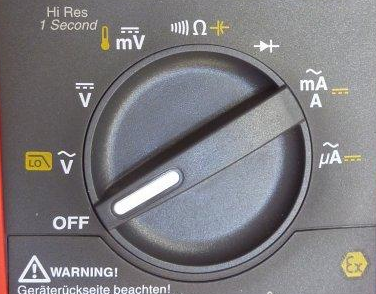
\includegraphics[scale=0.4]{Fluke28-II-switches}%% Dimensões e localização
    \fonte{\cite{flukeforum}}%% Fonte
\end{figure}

\section{Power Management}\label{powerManagement}

Multímetros digitais se apresentam em duas configurações, sendo estas de bancada e portátil. Na configuração portátil, se é utilizado pilhas ou baterias para prover a tensão necessária para se ligar todos os subsistemas do aparelho. Já na configuração de bancada, é utilizada uma fonte isolada, conectada à rede de energia para fornecer a tensão adequada para se ligar todos os subsistemas do dispositivo, como se pode ver nas figuras \ref{fig:batbt} e \ref{fig:bathh}, dos designs propostos pela \gls{TI}.

\begin{figure}[htb]%% Ambiente figure
    %\captionsetup{width=0.55\textwidth}%% Largura da legenda
    \caption{Diagrama de Blocos de um Multimetro Portátil}%% Legenda
    \label{fig:bathh}%% Rótulo
    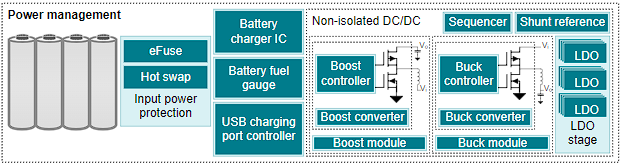
\includegraphics[scale=0.4]{bathh}%% Dimensões e localização
    \fonte{}%% Fonte
\end{figure}

\begin{figure}[h]%% Ambiente figure
    %\captionsetup{width=0.55\textwidth}%% Largura da legenda
    \caption{Diagrama de Blocos de um Multímetro de Bancada}%% Legenda
    \label{fig:batbt}%% Rótulo
    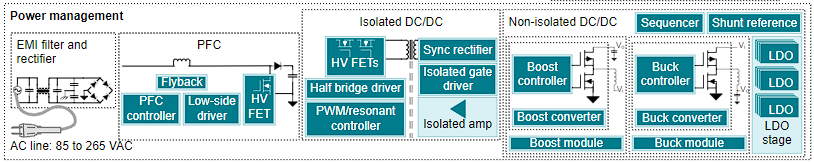
\includegraphics[width=1\textwidth]{batbt}%% Dimensões e localização
    \fonte{Texas Instruments}%% Fonte
\end{figure}

Existem vários modos de se projetar uma fonte adequada ao sistema proposto, mas para o escopo desta tese, foi optado por se utilizar uma fonte comercial que será escolhida para atender as necessidades do protótipo em questão.


% ANDREY------------------------------------------------------------------------

\section{Aquisição de Sinal}\label{sec:aqSignal}

A aquisição de sinal é o processo de captura e conversão de sinais físicos em um formato adequado para análise, processamento ou armazenamento. No contexto da medição de tensão e corrente, a aquisição de sinal refere-se à captura e registro desses parâmetros elétricos em um sistema de medição, permitindo sua análise, processamento ou armazenamento em um formato adequado.
Essa pode ser realizada de diferentes maneiras, dependendo do caso. Em alguns cenários, utiliza-se sondas específicas para cada aplicação, as quais permitem capturar e registrar os parâmetros elétricos de forma precisa. Por outro lado, em certos casos, a aquisição ocorre internamente dentro do circuito do próprio medidor, proporcionando uma solução integrada e simplificada para a captura e registro dos sinais elétricos.

\subsection{Resistor Shunt}\label{subsec:resiShunt}
Neste tipo de medição, um resistor de valor extremamente baixo (< 0,1 $\Omega$) é colocado em série com o circuito no qual se deseja medir a corrente elétrica, quando esta atravessa o componente, ocorre uma queda de tensão proporcional. Essa queda de tensão pode ser então medida diretamente através de um \gls{ADC} ou amplificada e então medida para se obter os valores da corrente original. \citep{curr_sens_tech}

Para a aplicação em 3 canais independentes de corrente, torna-se necessária algum tipo de isolação. Isso pode ser obtido utilizando-se de amplificadores isoladores --- amplificadores operacionais que possuem duas referências isoladas entre si. Permitindo uma medição da queda de tensão sobre o resistor shunt para cada canal sem interferência mútua, como exemplo o AD202 na \autoref{AD202}.

\begin{figure}[htb]
    \caption{AD202 um exemplo de amplificador isolador}
    \label{AD202}
    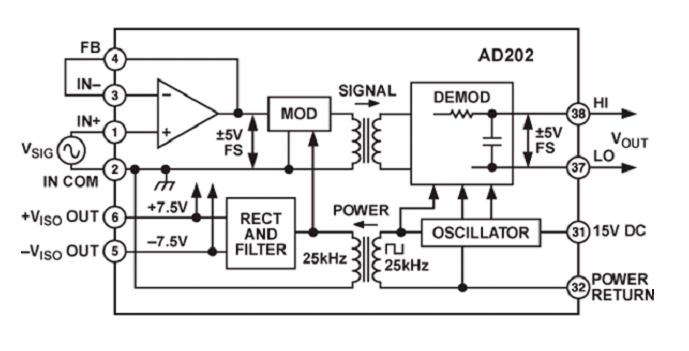
\includegraphics[width=0.8\textwidth]{figuras/AD202-ampop-isolado.png}
    \fonte{\cite{ad202}}
\end{figure}
    
Esse tipo de amplificador, porém, apresenta alto custo e possui uma variação de leitura considerável com a temperatura. São inferiores em precisão a outros métodos de medição que realizam o isolamento do circuito inerentemente por seus aspectos construtivos. 

\subsection{Bobina Rogowski}\label{subsec:Rogowski}

Utilizando-se do princípio da Lei da Indução de Faraday, a bobina Rogowski trata-se de um loop fechado de fio enrolado em volta de um aro. Esse aro envolve o condutor que, por sua variação de corrente, induz uma tensão elétrica proporcional ao número de espiras e a intensidade da própria corrente a ser medida. Para a medida dos valores obtidos pela bobina Rogowski, é necessário o uso de um integrador (por vezes acoplado no próprio cabo da ponteira de medição) para relacionar a derivada da corrente com a tensão obtida em seus terminais, podendo causar certo erro introduzido pela operação.

\begin{figure}[htb]
    \caption{Bobina Rogowski aberta}
    \label{fig:rogowski-bobina}
    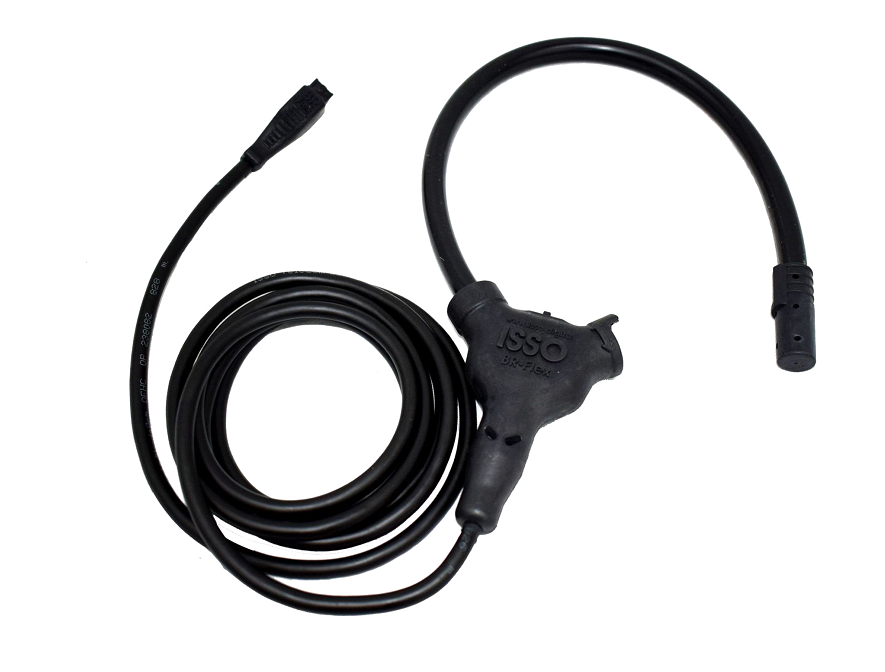
\includegraphics[width=0.8\textwidth]{figuras/bobina-rogowski.png}
    \fonte{CITAR Metodos de medição (artigo)}
\end{figure}

É um método amplamente utilizado para medições de altas correntes e suporta uma grande faixa de frequências. Tem um custo próximo dos transformadores de corrente e insere menos impedância parasita no circuito. \citep{curr_sens_tech}

\subsection{Transformador de Corrente}\label{subsec:t-corrente}

O princípio de funcionamento do transformador de corrente é parecido com o da bobina Rogowski: possui um primário e um secundário com uma razão de voltas que permite que a tensão induzida seja lida em sua saída. A diferença deste para a bobina Rogowski é que existe agora um núcleo com certa permeabilidade magnética e o secundário possui um resistor Rs que permite uma medição mais simplificada da corrente de entrada.
Nesse tipo de medição, a própria saída do transformador de corrente é proporcional a entrada de corrente, não sendo necessário um integrador como é o caso da bobina Rogowski. Devido a sua construção, seu sinal de saída também não necessita de nenhum tipo de amplificação, podendo ser lido diretamente por um \gls{ADC}. É teoricamente impossível medir correntes contínuas com esse método, porém, caso seja possível pulsar essa corrente, utilizando um circuito acessório de desmagnetização e, respeitando os tempos necessários entre os pulsos, é possível obter uma medida satisfatória.

\begin{figure}[htb]
    \caption{Circuito completo com transformador de pulso para medição \gls{CA}/\gls{CC}}
    \label{fig:circuito-tc-dc}
    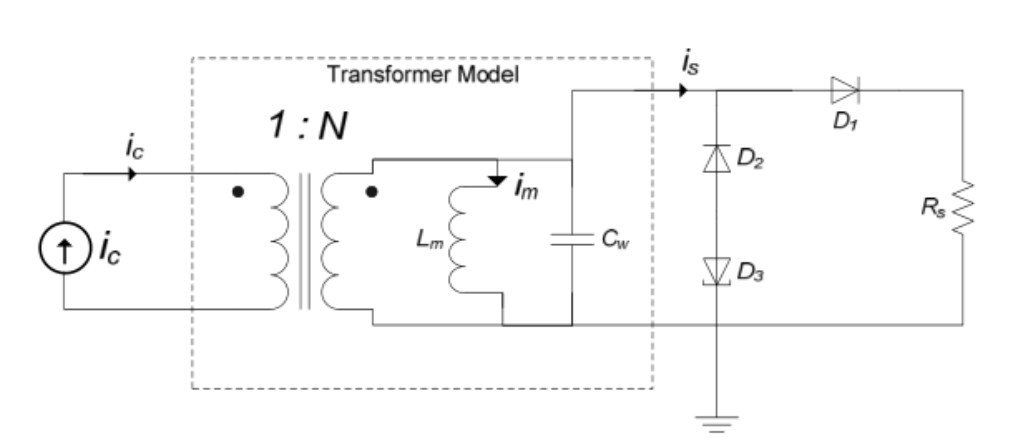
\includegraphics[width=0.8\textwidth]{figuras/transform-corrente-dc.png}
    \fonte{\cite{curr_sens_tech}}
\end{figure}

\subsection{Circuito Integrado de Medição \textit{(hall effect)}}\label{subsec:halleffect}

Existem circuitos integrados capazes de medir a corrente alternada de maneira isolada do
restante do circuito. Utilizando-se do efeito hall, o campo magnético gerado pela corrente
que passa entre seus terminais é medida por um sensor montado diretamente no substrato
do chip. Uma tensão proporcional a esse campo é fornecida pelo CI como saída e pode ser
medida por um ADC, recuperando-se o valor da corrente original.
O uso dessa tecnologia traz custo baixo em relação ao uso de TC's ou bobinas Rogowski,
fácil implementação no sistema, isolamento diretamente no chip.
Tal medição, porém, possui uma resolução na ordem de \SI{100}{\milli\volt\per\ampere} (considerando um CI que suporte acima de 10 A) e um ruído intrínseco de 11 mV. Como é o caso do ACS712.\citep{acs712}

\section{Aviso de Entrada Incorreta \textit{(Input Warning)}}\label{sec:inpWarning}

O termo \textit{input warning} refere-se a um aviso emitido quando ocorre uma entrada incorreta ou anormal em um sistema de medição. Esse tipo de aviso é acionado quando há um problema que pode afetar a precisão ou confiabilidade dos dados de medição. Pode ser uma condição fora dos limites esperados, como valores de tensão ou corrente que ultrapassam os limites especificados pelo instrumento de medição. \cite{base_alarms}

Em medições de tensão e corrente em um único canal, um aviso de entrada incorreta pode ocorrer quando os valores medidos excedem os limites estabelecidos pelo instrumento. Por exemplo, se a tensão medida estiver além da faixa de operação máxima, o aviso é acionado para indicar que a medição está fora dos limites aceitáveis.

Em medições com vários canais, o \textit{input warning} pode ser diferenciado dependendo da configuração do sistema de aquisição de dados. Pode haver avisos específicos para cada canal, indicando problemas individuais, como tensão excessiva ou corrente anormalmente alta. Alternativamente, pode haver um aviso global indicando um problema geral em qualquer um dos canais.

\subsection{Comparador para detecção de falhas} \label{subsec:compfalhas}

Para o caso do multímetro a ser desenvolvido pode-se utilizar um simples circuito comparador para monitorar as tensões de entrada e indicar ao usuário que a escala utilizada está incorreta ou, até mesmo, que a tensão ou corrente medidas está acima do limite suportado. O circuito pode ser visto na \autoref{fig:comparador-simples} e consiste apenas em um \gls{amp-op}.

\begin{figure}[htb]
    \caption{Circuito de um comparador utilizando dois resistores como referência de tensão}
    \label{fig:comparador-simples}
    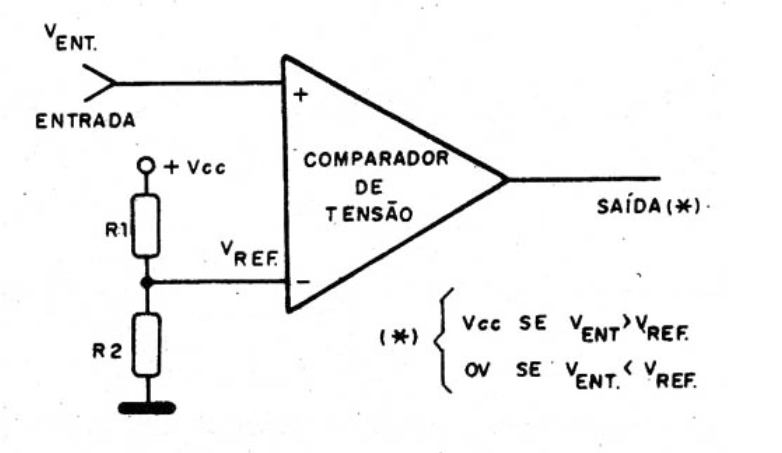
\includegraphics[width=0.8\textwidth]{figuras/ampop-comparador.png}
    \fonte{\cite{comp_ncbraga}}
\end{figure}

Dessa maneira, uma vez definida a tensão de referência, pode-se utilizar-se da saída para disparar algum tipo de aviso.

\subsection{Tipos de aviso} \label{subsec:tiposdeaviso}

Os avisos podem ser luminosos, sonoros, ou até mesmo gerar vibrações ou movimentações mecânica mais rigorosas a fim de afastar ou notificar o usuário do dispositivo.\cite{base_alarms}

Para tanto, em casos mais brandos --- onde há o uso da escala incorreta do medidor --- pode-se utilizar uma luz de aviso. Dado que esse uso não danifica o dispositivo, apenas impossibilita a leitura correta do dado.
Em casos mais sérios, onde há a possibilidade de causar dano ao aparelho de medição ou até mesmo ao usuário, se faz necessário um aviso mais severo, como, por exemplo, uma sirene alta.

\subsection{Casos de extrema gravidade} \label{subsec:casosextrgraves}

Um erro comum em laboratórios de eletrônica é a tentativa de medição de tensão elétrica utilizando-se do modo de medição de corrente elétrica do dispositivo. 

Comumente a corrente é medida através da queda de tensão em um resistor \textit{shunt}, conforme discorrido em \ref{subsec:resiShunt}. Colocar as ponteiras em um ponto onde haja tensão sem nenhum dispositivo limitador de corrente, faria com que o resistor shunt sofresse um enorme estresse levando possivelmente a sua falha ou diminuição drástica da vida útil.

Como geralmente há um sistema de proteção nesses dispositivos, muitas vezes, há a queima de um elemento fusível no lugar do resistor shunt. Porém, é necessário alertar o usuário de que o uso do equipamento foi incorreto e, caso a corrente seja removida a tempo, preservar a própria proteção. Caso essa seja rompida, também é importante notificar o usuário de que a mesma deve ser substituída.

Para tanto, pode-se utilizar um \textit{buzzer} com o som alto o suficiente para notificar o usuário mesmo em um ambiente com certo ruído, como é o caso de um laboratório de aula. 

% Removida essa seção, não foi encontrado nada de muito útil que pudesse ser efetivamente usado. Trata-se apenas de um sistema para proteger o MCU em alguns casos específicos.
%%\section{Isolador de sinal digital \textit{(Digital Signal Isolator)}}\label{sec:DSIsolator}


\section{MCU e Interface de Comunicação}\label{sec:MCUInterface}

\subsection{Microcontroladores}\label{subsec:MCU}

O \gls{MCU} ou \textit{Microcontroller Unit} é um dispositivo eletrônico altamente integrado contendo um processador, memória e periféricos de entrada e saída. Os microcontroladores são amplamente utilizados em uma variedade de aplicações, desde eletrodomésticos e automóveis até dispositivos médicos e sistemas de controle industrial.

Ele é projetado para ser compacto, de baixo consumo de energia e fácil de programar. Eles são usados para controlar e executar tarefas específicas em um sistema eletrônico. Ao contrário de um microprocessador, que é projetado para executar uma ampla variedade de tarefas e requer componentes externos adicionais, o \gls{MCU} possui praticamente todos os recursos necessários integrados em um único chip.

No caso dos medidores, o \gls{MCU} é utilizado como o interpretador dos sinais obtidos pelo \gls{ADC}, podendo realizar as operações matemáticas necessárias para se obter os valores médios, eficazes, pico, e demais necessários, a partir da amostragem obtida. Esse é o caso do \textit{3Ph-ozm}, que utiliza um microcontrolador com pré-processador dos dados e como sistema de controle para as funções fundamentais do dispositivo. \cite{3ph-ozm}

Juntamente do \gls{MCU}, o \textit{3Ph-ozm} utiliza um microprocessador para realizar o trabalho de comunicação através de WiFi e Bluetooth.
Tal abordagem, porém, traz um custo mais alto ao projeto, uma vez que um microprocessador é mais caro que um microcontrolador --- que pode ser capaz de tanto processar, como enviar os sinais. \cite{uCdiff}

\subsubsection{Microcontroladores Considerados} \label{subsubsec:uc-disp}

Existe uma vasta gama de \gls{MCU}'s capazes de realizar o processamento dos sinais obtidos. Logo, se faz necessária uma filtragem prévia dos principais requisitos do projeto antes mesmo do inicio da metodologia.
Para tanto, foram considerados os seguintes pontos:

\begin{itemize}
    \item Popularidade --- um item popularmente conhecido pode ser encontrado com maior facilidade em lojas locais;
    \item Facilidade de programação --- como um dos objetivos primordiais do projeto é a replicabilidade e a disponibilização por meios \textit{open source}, a simplicidade na programação deve ser levada em conta;
    \item Preço --- o microcontrolador tem potencial para ser o item único mais custoso do projeto, reduzir seu preço auxiliaria na questão do baixo custo;
    \item Capacidade de processamento --- devido o tratamento de três canais em simultâneo e/ou do uso de comunicação por WiFi ou Bluetooth, se faz necessária uma solução que tenha capacidade de processamento de acordo
\end{itemize}

Seguindo esses critérios e as informações disponíveis no artigo \textit{How to Select the Microcontroller for Your New Product} \cite{select_uC}, os \gls{MCU}'s adequados à finalidade de medição seriam os que possuem arquitetura de 32 bits, uma vez que estes possuem também certas características de microprocessadores como, por exemplo, a lógica de prioridade nas interrupções e a velocidade de trabalho com ponto flutuante.

Os \gls{MCU}'s mais populares dessa arquitetura são os da família STM32.

\begin{figure}[htb]
    \caption{Família STM32 separada por função}
    \label{fig:stm32-family}
    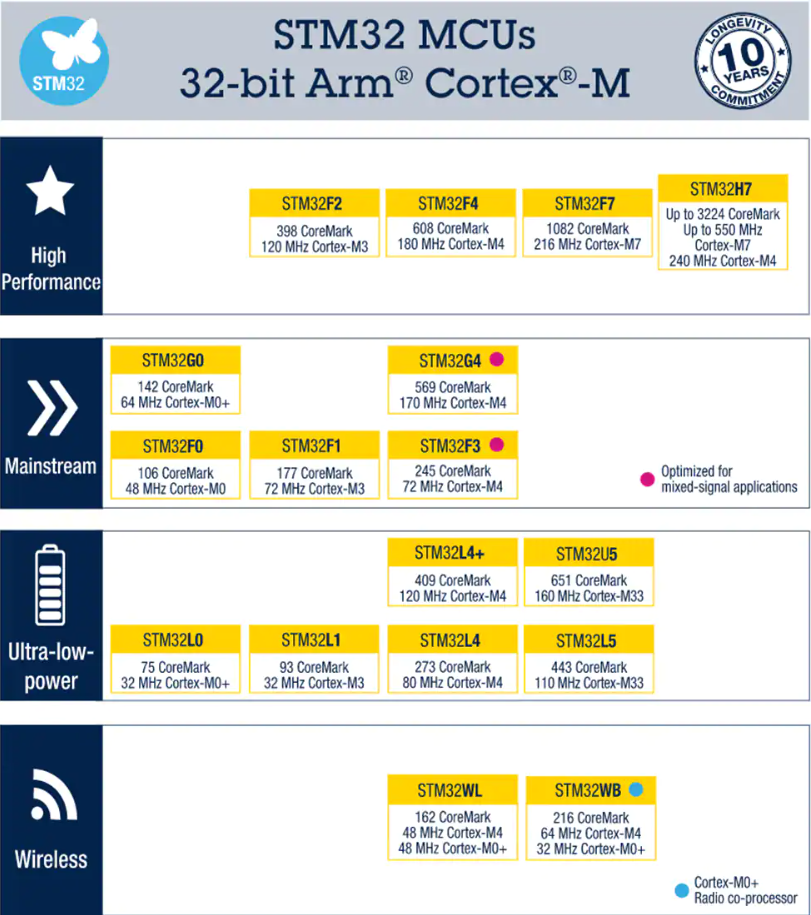
\includegraphics[width=0.7\textwidth]{figuras/STM32-family.png}
    \fonte{Mouser}
\end{figure}

Para a seleção de um microcontrolador adequado, pode-se seguir a linha \textit{mainstream} da \autoref{fig:stm32-family}, pois tratam-se de \gls{MCU}'s populares e que possuem vasta documentação disponível online.

\subsection{Interface de Comunicação}\label{sec:Interface}

Os dispositivos de medição que possuem comunicação com sistemas externos o fazem de diversas maneiras. 

A mais simples delas trata-se de um display que apresenta os valores da leitura ao usuário. Este pode utilizar a tecnologia de \gls{LCD} ou semelhantes para mostrar apenas números, como também pode mostrar as formas de onda em telas que possuam uma resolução maior.

Os dados também podem ser enviados a um sistema externo que fará a apresentação dos dados, os armazenará para usos posteriores, ou dará outra finalidade conforme o sistema.

Para realizar esse envio, podem-se utilizar diversas tecnologias diferentes, desde protocolos com fio (CAN, MODBUS, I2C, UART, etc.) até protocolos sem fio --- que serão os mais aprofundados nessa seção.

Baseando-se no artigo \citet{lowcost-smartmeter}, as tecnologias que podem ser usadas são as encontradas no ambiente de IoT (Internet das Coisas) como LoRa, Sigfox e NB-IoT. Também é possível utilizar tecnologias mais populares, como é o caso do \citet{3ph-ozm} que utiliza WiFi e Bluetooth para realizar sua comunicação e o display de seus dados através de uma interface web conforme a \autoref{fig:interface-3ph-ozm}.

\begin{figure}[htb]
    \caption{Interface WEB usada no 3Ph-ozm}
    \label{fig:interface-3ph-ozm}
    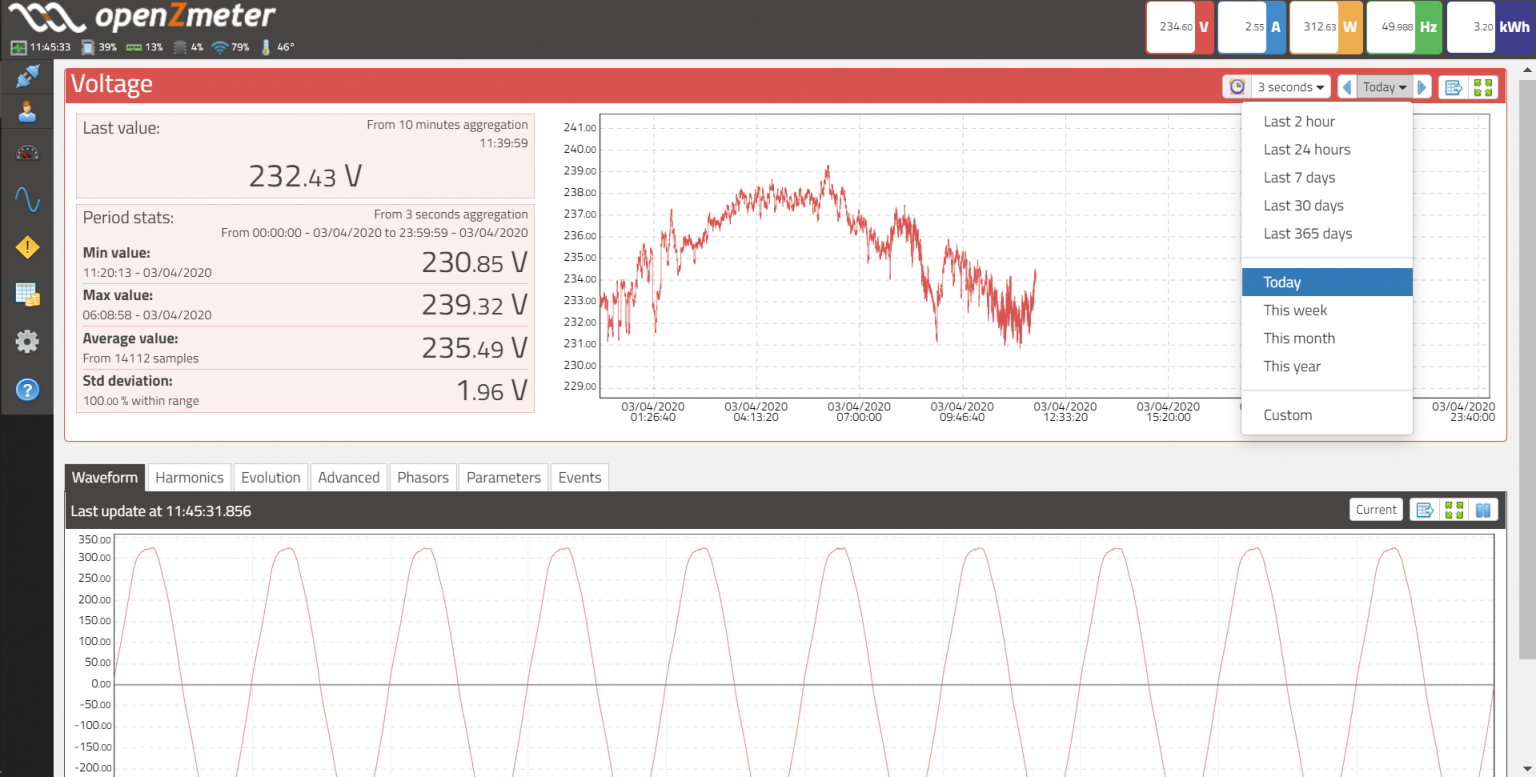
\includegraphics[width=0.9\textwidth]{figuras/interface-web-openzmeter.png}
    \fonte{www.openzmeter.com/}
\end{figure}

\subsection{Soluções completas}\label{subsec:solucomp}

Há também a possibilidade da utilização de módulos que possuem um microcontrolador e outras funções integradas. Como é o caso do ESP32-WROOM-32D (\autoref{fig:esp32-frente-verso}), construído em torno do chip ESP32.

Esse módulo possui um microprocessador \textit{Xtensa® Dual-Core 32-bit LX6} e as funções principais de um microcontrolador, como \gls{ADC} próprio e tratamento de interrupções por ordem de relevância. Além de possuir dois \gls{DAC}'s. O principal diferencial desse módulo, porém, é a sua capacidade de trabalhar com WiFi e Bluetooth sem a necessidade de nenhum periférico extra, além de possuir grande facilidade em sua programação. \cite{esp32-datasheet}

\begin{figure}[htb]
    \caption{Módulo ESP32-WROOM-32D frente e verso}
    \label{fig:esp32-frente-verso}
    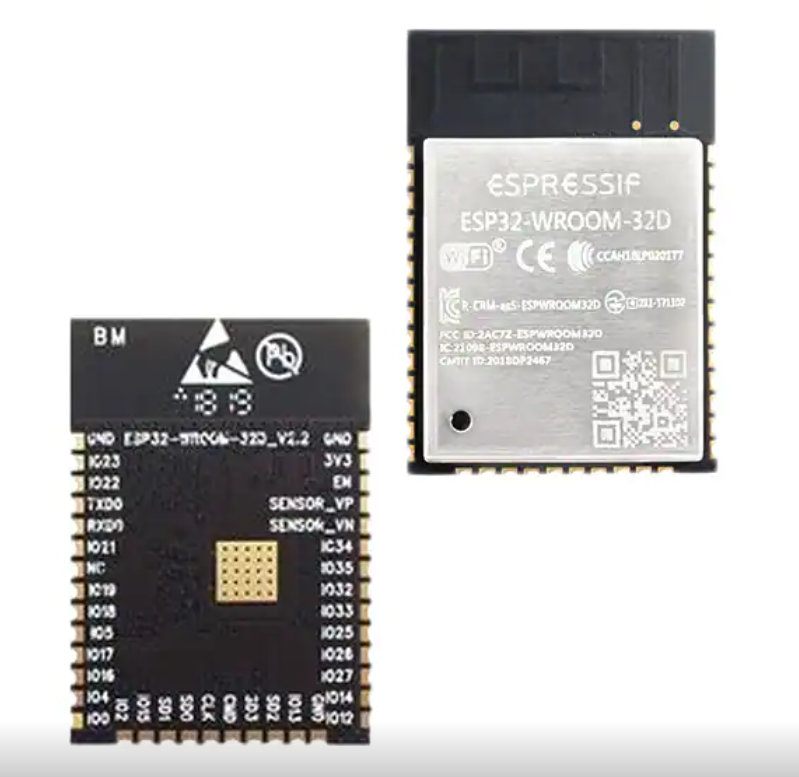
\includegraphics[width=0.3\textwidth]{figuras/esp32-frente-verso.png}
    \fonte{DigiKey}
\end{figure}